\documentclass{article}\usepackage[]{graphicx}\usepackage[]{color}
%% maxwidth is the original width if it is less than linewidth
%% otherwise use linewidth (to make sure the graphics do not exceed the margin)
\makeatletter
\def\maxwidth{ %
  \ifdim\Gin@nat@width>\linewidth
    \linewidth
  \else
    \Gin@nat@width
  \fi
}
\makeatother

\definecolor{fgcolor}{rgb}{0.345, 0.345, 0.345}
\newcommand{\hlnum}[1]{\textcolor[rgb]{0.686,0.059,0.569}{#1}}%
\newcommand{\hlstr}[1]{\textcolor[rgb]{0.192,0.494,0.8}{#1}}%
\newcommand{\hlcom}[1]{\textcolor[rgb]{0.678,0.584,0.686}{\textit{#1}}}%
\newcommand{\hlopt}[1]{\textcolor[rgb]{0,0,0}{#1}}%
\newcommand{\hlstd}[1]{\textcolor[rgb]{0.345,0.345,0.345}{#1}}%
\newcommand{\hlkwa}[1]{\textcolor[rgb]{0.161,0.373,0.58}{\textbf{#1}}}%
\newcommand{\hlkwb}[1]{\textcolor[rgb]{0.69,0.353,0.396}{#1}}%
\newcommand{\hlkwc}[1]{\textcolor[rgb]{0.333,0.667,0.333}{#1}}%
\newcommand{\hlkwd}[1]{\textcolor[rgb]{0.737,0.353,0.396}{\textbf{#1}}}%

\usepackage{framed}
\makeatletter
\newenvironment{kframe}{%
 \def\at@end@of@kframe{}%
 \ifinner\ifhmode%
  \def\at@end@of@kframe{\end{minipage}}%
  \begin{minipage}{\columnwidth}%
 \fi\fi%
 \def\FrameCommand##1{\hskip\@totalleftmargin \hskip-\fboxsep
 \colorbox{shadecolor}{##1}\hskip-\fboxsep
     % There is no \\@totalrightmargin, so:
     \hskip-\linewidth \hskip-\@totalleftmargin \hskip\columnwidth}%
 \MakeFramed {\advance\hsize-\width
   \@totalleftmargin\z@ \linewidth\hsize
   \@setminipage}}%
 {\par\unskip\endMakeFramed%
 \at@end@of@kframe}
\makeatother

\definecolor{shadecolor}{rgb}{.97, .97, .97}
\definecolor{messagecolor}{rgb}{0, 0, 0}
\definecolor{warningcolor}{rgb}{1, 0, 1}
\definecolor{errorcolor}{rgb}{1, 0, 0}
\newenvironment{knitrout}{}{} % an empty environment to be redefined in TeX

\usepackage{alltt}

\title{Videography and the Santa Ana Sucker}
\author{Clare Flynn and Wendy Norena}
\IfFileExists{upquote.sty}{\usepackage{upquote}}{}
\begin{document}
\SweaveOpts{concordance=TRUE}

\maketitle

\newpage
\tableofcontents
\newpage

\section{Introduction}
The Santa Ana sucker is a 16 cm fish that lives in the rivers of Southern California.  They have recently been placed on the endangered species list, partially due to their losing over 70 percent of their habitat (FWS 2012). Also, in the 1960s, the habitat of the suckers would range from 10-26°C, but when we tested the water in September 2016, we found temperatures in the Santa Ana river up to 35.5°C (Greenfield & Ross & Deckert 1970).  This rise in temperature is most likely due to the extreme industrialization of the stream; much of it runs over concrete, which heats up to extreme temperatures in the sunlight.  A majority of the stream water also comes from discharge from a sewage treatment plant upstream, creating an unhealthy and unnatural environment.  The river is also greatly diminished from what it used to be due to the extreme drought in Southern California.  The river is shallower, slower moving, and has less ice melt coming from the mountains, all of which factor into an increase in temperature.  Our goal of this study is to discover whether or not the Santa Ana suckers are coping with this dramatic increase in temperature by moving to cooler sections of the stream throughout the day.  
Greenfield, D. W., Ross, S. T., & Deckert, G. D. (1970). Some aspects of the life history of the Santa Ana sucker, Catostomus (Pantosteus) santaanae (Snyder). Calif. Fish Game, 56(3), 166-179.
USFWS (2012, March). Recovery Outline for Santa Ana Sucker (Catostomus santaane). U.S. Fish and Wildlife Service. Retrieved October 10, 2016, from https://www.fws.gov/carlsbad/tespecies/Recovery/documents/Recovery Outline for Santa Ana Sucker-3-30-2012.pdf.


\subsection{Problem Statement}
Does the Santa Ana Sucker shift its distribution in the Santa Ana River based on natural temperature changes that occur throughout the day? We believe that if we monitor the relative distribution of the Santa Ana Suckers throughout the day we will see a difference in sucker abundance between an upstream and downstream location in response to changing temperature throughout a 24-hour period.

\subsection{Background (Literature Review)}
We expect that water temperatures at the downstream location will be less than the upstream location throughout the day. We know the current range of the Santa Ana Sucker differs significantly from its historic distribution in the Los Angeles Basin (Thompson 2010). We also know that the sucker prefers environments with cool water (Moyle 2002) and other fish have been known to regulate their body temperatures by moving to different areas in their habitat throughout the day (Matthews & Berg & Azuma 1994)

\subsection{Objectives}
Our goal is to obtain footage clearly showing the density of Santa Ana suckers in the different locations at different points in the day.  We hope to get accurate enough footage to count the number of fish in each video, then run an ANOVA test on each location to see if the quantity of fish significantly varies at different times of the day.  If they do, we will be able to conclude that the suckers move throughout the day to find their preferred temperature.

\subsection{Materials and Equipment}
\begin{itemize}
\item 2 Waterproof GoPro Hero 4 Silver cameras with mounts
\item 4 64GB microSD SanDisk memory cards
\item 4 Waterproof Re-Fuel 6-Hour ActionPack Battery for GoPro HERO by DigiPower
\item 2 HOBO Tidbit water temperature data loggers
\item 2 Grey Cinder block cubes open on two parallel sides, ~8in x 8in x 8in, Home Depot
\item 2 Grey Cinder block backs, ~8in x 8in
\item 1 bottle of Original Sticks to Everything Gorilla Glue
\end{itemize}



\section{Methods}
We acquired all the necessary equipment for an underwater filming project, keeping in mind the length of time we wanted to keep our cameras underwater. We chose the GoPro Hero 4 Silver because of its battery life and recording time. We also considered safety and theft prevention for the cameras, and for this reason decided to mount the cameras in cube-shaped cinderblock structures with one open side that we constructed ourselves. In the lab, we set up all the equipment, built the cinderblock structures, and prepared everything for the field. Once in the field, we selected appropriate data sites, set up our cameras, and placed them at certain specific times of the day. More detailed information on these processes can be found in the following sections.

\subsection{Site Description}
 We collected our video on-site at the Santa Ana River. As a class we chose to collect data from four points along a small stretch of the river that was easily accessible by car. Because of this, the part of the river we took data from was relatively close to roadways and traffic. 
The specific sites for our project consisted of one upstream location (site 2) and one downstream location (site 4), located roughly one kilometer apart. Site 2 was located just below the Rialto concrete channel and site 4 was a plunge pool. The upstream location was significantly more encumbered with large debris like rocks and branches. The downstream location was smooth and flat, with a bed of pebbles and smaller coarse sediments (Figure \ref{SAR_Image}). 

\begin{figure}
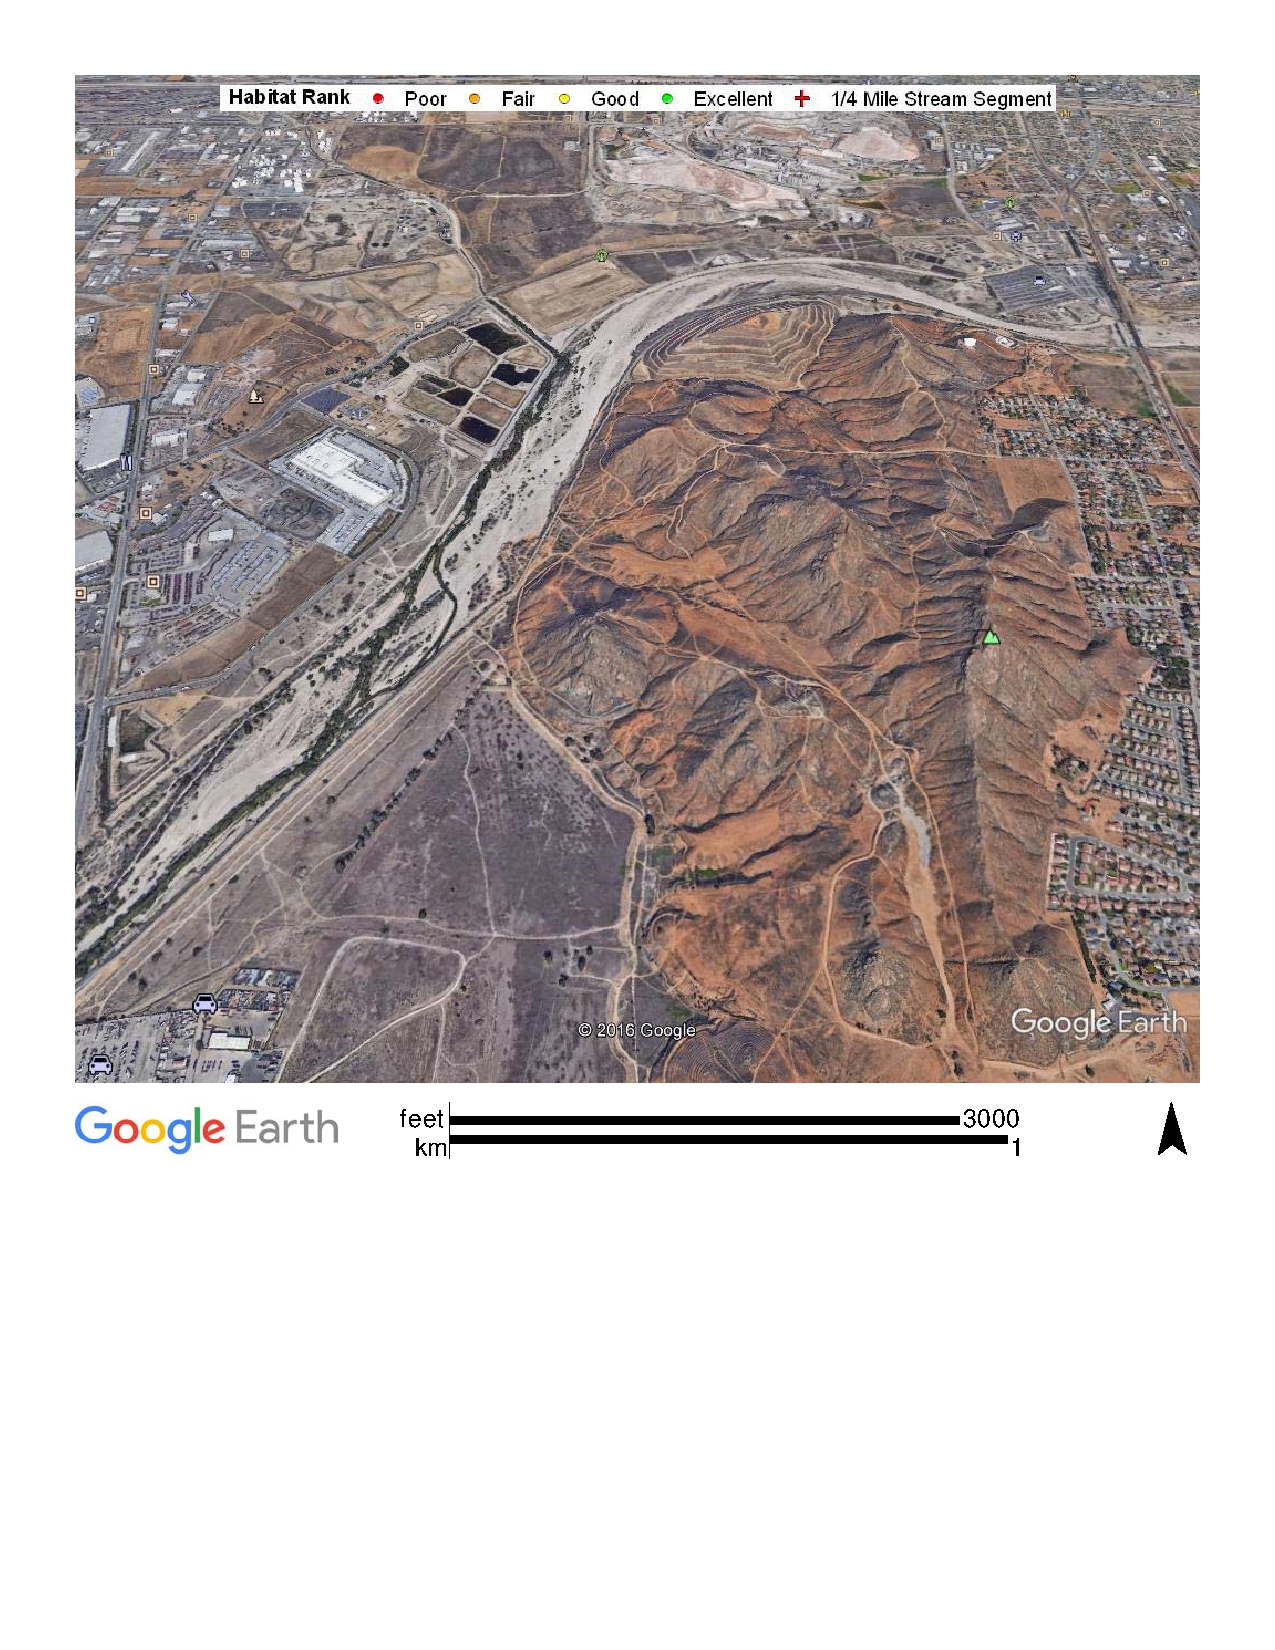
\includegraphics[width=1.00\textwidth]{Figures/SantaAna_SatelliteImage}
\caption{Google Earth --Example of a map. What's wrong with this image?}
\label{SAR_Image}
\end{figure}

\subsection{Laboratory Methods}
To set up the cameras, we removed them from the packaging, inserted a microSD card into each, and charged them fully by connecting the included USB cables to a computer. The cameras needed to be fully charged before we were able to adjust the settings. Once the cameras were sufficiently charged, we set the filming settings to record in 720p x 30fps. We set the cameras aside and left them charging. 
Next, we charged all four of the waterproof Re-Fuel battery packs. As these were charging, we put together our cinder block mounting structures. We took our cinder block cubes and set them up on a clean, stable table. We connected the flat adhesive mounts that were included with the GoPros and connected a GoPro camera to each. Since the cinder blocks were open on two parallel sides, we were able to see right through the cinder block cube to the other side. One of us stood on one side with the GoPro and mount, and the other stood on the other side of the opening. One of us turned the GoPro on and put the camera with the mount inside the cinder block cube, using the view on the screen to find the best position for the mount inside of the cube, taking care to ensure we could clearly see the other person on the other side. We found an ideal place where the view was mostly unobstructed by the sides of the cube but the cameras were still far enough inside the cube that they wouldn’t be too easily spotted by passersby. This spot was 5 cm from the edge of the cube. We traced the front and the back of the mount so we could glue it in the correct place. We repeated this procedure for the second cube and mount, and standardized the construction by placing the mount in the second cube 5 cm away from the edge of the cube. 
In order to securely glue the mount in place, we used Gorilla glue. To activate the Gorilla glue, we first had to moisten one of the surfaces with water. We moistened the mounts on the adhesive side. We did not remove the adhesive backing so we could reutilize the mounts in the future. Once the mount was damp, we put Gorilla glue on the cinder block inside the lines we had drawn around the mount. We then placed the mount on the Gorilla glue, taking care to align the edges of the mount with the lines we had drawn. Next, as per the Gorilla glue instructions, we found a heavy object that could provide significant pressure on the mount and that would fit inside the cube. We left this for three hours to harden.
Upon returning to the lab, we removed the heavy objects from the cube and checked the seal on the mount and cinder block to ensure the bond had successfully cemented. After this, we went to work on attaching the cinder block backs to close up one of the open sides on the cubes. We repeated much of the same process we used when attaching the mounts to the cubes, and followed the Gorilla Glue instructions carefully. First, one of us moistened the cinder block back while the other applied Gorilla Glue to the edge of the cube. Then, we carefully aligned the corners of the back with the cube. We repeated this with the second cube. Seeing that the cinderblock back was heavy enough on it’s own, we did not place a heavy object on top of this structure and instead simply left it to dry and harden overnight.
Finally, we checked on the cameras and battery packs again to ensure they had charged. We left them plugged in overnight. We also packed away the Gorilla Glue, the multiple SD cards, paper towels, and extra mounts in a field kit so we could deal with any emergencies in the field. 

\subsection{Field Methods}
We started our first recording session at 10 am.  We drove to the downstream site and found a spot under brush cover in a pool next to a fast moving section of the stream.  We first placed the cinderblock squarely on the riverbed and positioned it facing the fast moving water.  We then turned the camera on, pressed record, and placed it on the mount in the cinderblock.  We let it run for a few seconds, then took it out and watched the video to ensure it was recording at a good angle.  We then pressed record again and replaced it.  Before leaving, we marked the area with flags so we would be able to find it again.
Next, we walked approximately 20 minutes upstream to another covered pool next to a fast moving section, and repeated the camera placement procedures.  We marked with flags, and then left.
We returned at approximately 2 pm.  We took out the camera at the downstream site, replaced the memory card and the battery pack, hit record, and replaced the camera exactly as it was positioned previously.  We then walked upstream and did the same thing with the second camera.  After returning, we cleared the memory cards and plugged in the battery packs.
Our last recording session was at 8 am the next morning.  We replaced the memory cards and battery packs again and returned the cameras to their positions.  One of us returned the next day to collect the cameras.


\subsection{Statistical Methods}
We ran an ANOVA test where time period was the categorical independent variable and number of fish was the continuous dependent variable.  We weren’t able to run the test for location 2 because there were too few fish seen to draw any conclusions.  We also couldn’t test the effect of location on number of fish, because the conditions were too different between the upstream and downstream locations to compare.

\section{Results}
We counted an average of 20.133 suckers in the morning with a standard deviation of 6.007 fish.  In the afternoon, we counted an average of 32.25 with a standard deviation of 9.928, meaning both the average and the variance were higher in the afternoon.  The river was 27.764°C in the morning and increased to 28.456°C in the afternoon.  We calculated a p-value of 6.027e-13, which is less than .05 so we can reject our null hypothesis that tie of day will have no effect on the number of fish.
\begin{knitrout}
\definecolor{shadecolor}{rgb}{0.969, 0.969, 0.969}\color{fgcolor}\begin{kframe}
\begin{alltt}
\hlstd{newmetadata} \hlkwb{<-} \hlkwd{read.csv}\hlstd{(}\hlstr{"/home/CAMPUS/cmfa2015/Santa Ana Sucker/Data/Data_Tues_2/newmetadata.csv"}\hlstd{)}
\end{alltt}
\end{kframe}
\end{knitrout}
\begin{knitrout}
\definecolor{shadecolor}{rgb}{0.969, 0.969, 0.969}\color{fgcolor}\begin{kframe}
\begin{alltt}
\hlkwd{boxplot}\hlstd{(Fish}\hlopt{~}\hlstd{Section,newmetadata,} \hlkwc{ylab}\hlstd{=}\hlstr{"Fish"}\hlstd{,}\hlkwc{xlab}\hlstd{=}\hlstr{"Time of Day"}\hlstd{,}\hlkwc{main} \hlstd{=}\hlstr{"Time of Day as a predictor of Fish"}\hlstd{,}\hlkwc{las}\hlstd{=}\hlnum{1}\hlstd{)}
\end{alltt}
\end{kframe}
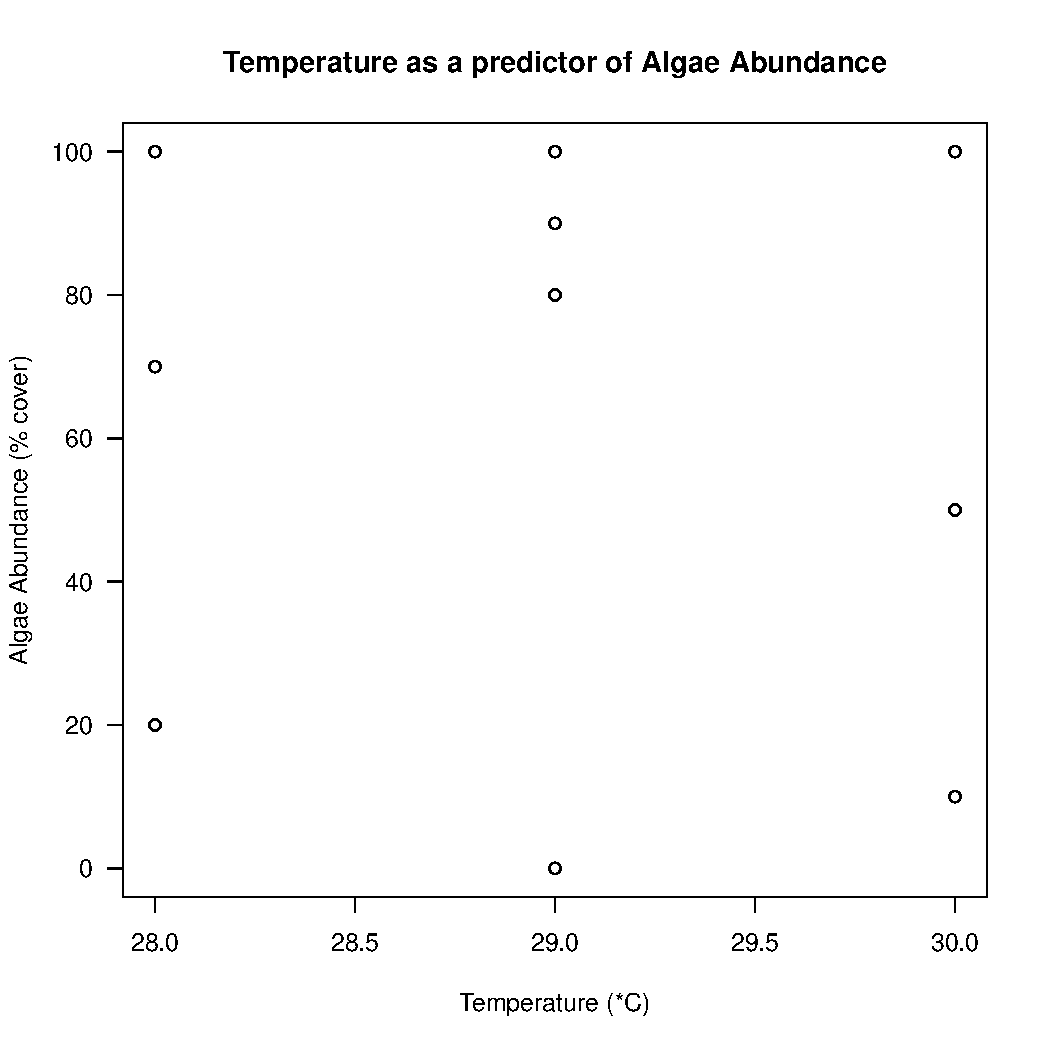
\includegraphics[width=\maxwidth]{figure/unnamed-chunk-2-1} 

\end{knitrout}
\begin{tabular}{ |p{1.5cm}||p{1cm}|p{1cm}|{p2cm}|{p2cm}|{p2cm}|{p2cm}|{p2cm}|  }
 \hline
 \multicolumn{8}{|c|}{Videography Summary Statistics} \\
 \hline
 Section & Min & Max & Mean & Median & 1st Quartile & 3rd Quartile & K\\
 \hline
 Morning & 7 & 29 & 20.13 & 22  & 16.75 & 25 & -0.6\\
 Afternoon & 14 & 49 & 32.25 & 31 & 24.75 &  42 & -1.3\\
 \hline
\end{tabular}

\section{Discussion}
Our videos of site 2 contained so few fish that we were unable to draw any conclusions from the data.  In the morning there were no Santa Ana suckers seen in the entire hour, and in the afternoon there was one sucker that would occasionally swim out from behind a rock.  This could be because the temperature that far upstream was too hot for the suckers to live there; the temperature data found that at that location the water was around 29°C in the afternoon and 25°C in the morning.  It is also possible that our camera was placed in a section of the river that the suckers don’t like, so the lack of fish could have had nothing to do with temperature.
When we compared the number of fish downstream in the afternoon compared to the morning, we had a p-value of 6.027e-13, meaning there were significantly more suckers in the afternoon than there were in the morning.  This suggests that the suckers do move downstream throughout the day to get to cooler temperatures.  On the afternoon we tested, the plunge pool (downstream) was 28.5°C, whereas the river at our upstream location, closer to the concrete, was 29.4°C.  However, we cannot definitively prove that we observed more fish in the afternoon because of the temperature change; there could have been a variety of other factors.  For example, the fish could have moved from one river bank to the other throughout the day to stay in the shade of the brush as the sun moved.


\section{Conclusion and Recommendations}
Based on our findings, it seems that the Santa Ana sucker could possibly migrate from upstream to downstream locations during the day in an attempt to regulate its body temperature. Further research is necessary to test this since we are unable to fully attribute the increase in fish in our afternoon footage to an intentional migration due to temperature changes in the water. 
If true, this finding could be useful in helping stakeholders design and implement successful conservation policies. Certain examples of this could be planting more trees on the riverbanks or requiring the sewage treatment plant to chill water before it’s released. Perhaps stakeholders could successfully acquire a larger conservation area for the fish that would allow the water to cool off over a longer distance and allow more room for the fish to migrate. 
Certain issues we ran into during our study included visibility and camera placement. Unfortunately, we did not formulate a standardized method with which to place our cameras in the water. For this reason, there were differences in footage from morning to afternoon as well as from site to site. For future studies, we recommend including physical place-markers in the river for the cinderblock structures, maybe in the form of flags placed directly in the river bed. Markers inside of the cinderblock structure that delineate the exact position and angle of the cameras would also be ideal in order to ensure that the same exact field of vision is present throughout the collected footage. Additionally, a marker such as a graphic scale would be useful to have in the camera’s field of vision in order to figure out size of the fish and distance from the camera. Finally, our model of GoPro did not have a timestamp feature. Though we were able to figure out the initial recording times from the data saved in each individual video file, a timestamp would have greatly facilitated and ensured the accuracy of our counting process.


For future studies of this sort, a longer data sampling process would be ideal. While we were only able to collect and analyze one hour of footage each for the morning and afternoon sections, a more robust study might have 20 or so hours each over the course of a single month. Perhaps even more data could be recorde than that, as there is no limit to the amount of data that could be taken for this study due to changes in season, water influx differences, and other factors, as well as the possibility of doing a temporal analysis on the density of the fish. 

\end{document}
